\documentclass[conference]{IEEEtran}
\IEEEoverridecommandlockouts
% The preceding line is only needed to identify funding in the first footnote. If that is unneeded, please comment it out.
\usepackage{cite}
\usepackage{amsmath,amssymb,amsfonts}
\usepackage{algorithmic}
\usepackage{graphicx}
\usepackage{textcomp}
\usepackage{xcolor}
\usepackage{float}
\usepackage{multirow}

% Label tabel dan gambar dalam bahasa indonesia
\renewcommand{\figurename}{Gambar}
\renewcommand{\tablename}{Tabel}

\def\BibTeX{{\rm B\kern-.05em{\sc i\kern-.025em b}\kern-.08em
    T\kern-.1667em\lower.7ex\hbox{E}\kern-.125emX}}
\begin{document}

\title{KENDALI \emph{MOBILE ROBOT} BERBASIS POSE TANGAN MENGGUNAKAN \emph{CONVOLUTIONAL NEURAL NETWORK} (CNN)
}

\author{\IEEEauthorblockN{1\textsuperscript{st} Alfan Miftah Arzaqi}
\IEEEauthorblockA{Departemen Teknik Komputer \\
Institut Teknologi Sepuluh Nopember\\
Surabaya, Indonesia \\
alfan.19072@mhs.its.ac.id}
\and
\IEEEauthorblockN{2\textsuperscript{nd} Ahmad Zaini, S.T., M.Sc.}
\IEEEauthorblockA{Departemen Teknik Komputer \\
Institut Teknologi Sepuluh Nopember\\
Surabaya, Indonesia \\
zaini@te.its.ac.id}
\and
\IEEEauthorblockN{3\textsuperscript{rd} Dr. Eko Mulyanto Yuniarno,S.T.,M.T.}
\IEEEauthorblockA{Departemen Teknik Komputer \\
Institut Teknologi Sepuluh Nopember\\
Surabaya, Indonesia \\
ekomulyanto@ee.its.ac.id}
}

\maketitle

\begin{abstract}
    Perkembangan teknologi \textit{Human Computer Interaction} atau HCI yang memungkinkan untuk berkomunikasi dengan komputer menggunakan pose tangan.dengan majunya teknologi suatu \textit{remote control} pada robot mulai dikembangkan dengan mengutamakan interaksi pengguna dengan robot. Sistem kendali pada robot sudah mulai meninggalkan \textit{remote control joystick} dan beralih pada kendali menggunakan gestur tangan atau secara \textit{autonomous}. Penggunaan \textit{remote control joystick} mulai ditinggalkan karena terdapat beberapa kekurangan dalam mengendalikan robot. Dalam penelitian ini dibuat kendali robot berbasis pose tangan menggunakan \textit{Convolutional Neural Network}. Pada penelitian ini \textit{remote control joystick} digantikan dengan kamera sebagai input pose tangan dari user. Citra yang ditangkap oleh kamera diklasifikasikan menggunakan \textit{Convolutional Neural Network} untuk menerjemahkan perintah dari pengguna kepada robot. Hasil klasifikasi diubah menjadi kode instruksi yang selanjutnya dikirimkan kepada robot menggunakan internet untuk diterjemahkan menjadi perintah navigasi oleh \textit{mikrokontroller}. Nilai akurasi yang didapatkan dari hasil \emph{training} menggunakan CNN sebesar 0.95 dan memiliki jarak ideal pada 50cm.
\end{abstract}

\begin{IEEEkeywords}
    \textit{Convolutional Neural Network}, \emph{Mobile Robot}, Pose,
\end{IEEEkeywords}

\section{Pendahuluan}
Pose adalah potongan-potongan dari gerakan yang bertujuan untuk komunikasi non verbal yang digunakan untuk menyampaikan pesan penting, baik secara langsung maupun tidak langsung tanpa menggunakan kata-kata. Setiap pose dapat memiliki arti tersendiri sesuai dengan kesepakatan umum ataupun personal yang melakukan komunikasi. Pose tangan berarti suatu sikap yang diberikan oleh tangan untuk berkomunikasi \cite{g1}. \par
Pose tangan ini biasa digunakan oleh penderita tuna rungu untuk berkomunikasi, namun dengan perkembangan teknologi dimana adanya teknologi \textit{human computer interaction} yang memungkinkan untuk berkomunikasi dengan komputer menggunakan pose tangan. \textit{Human Computer Interacttion} atau biasa disingkat HCI adalah suatu bidang studi yang merancanga teknologi komputer untuk lebih interaktif saat dipakai. Adanya HCI ini dapat memudahkan manusia untuk menyelesaikan tugas-tugasnya dengan bantuan komputer \cite{g4}. \par
Pada saat ini perkembangan HCI cukup pesat yang diakibatkan dari perkembangan pada teknologi \textit{machine learning} dan robotika. Teknologi \textit{machine learning} memungkinkan komputer untuk belajar dari data-data yang diberikan oleh manusia dan juga mengambil keputusan dari data-data tersebut. Pada salah satu cabang \textit{machine learning} yaitu \textit{computer vision} memungkinkan untuk komputer mengerti gerakan atau pose yang diberikan manusia melalui gambar atau vidio \cite{g3}. Tidak hanya \textit{machine learning} yang berkembang namun pada robotika juga berkembang terutama pada sistem kendalinya. Saat ini robot dapat dikendalikan tidak hanya menggunakan \textit{joystick}, namun juga dapat dikendalikan dengan gestur tangan dan juga secara  \textit{autonomous}, namun saat ini kendali menggunakan \textit{joystick} secara perlahan mulai ditinggalkan karena kurang memberikan pengalaman yang interaktif saat digunakan\cite{g2}. \par
Terdapat penelitian yang dilakukan oleh Fauzia \cite{g5} mengenai kendali robot menggunakan gestur tangan dengan bantuan alat yang ditempelkan pada punggung tangan. Kekurangan penelitian tersebut masih menggunakan alat yang ditempelkan pada tangan untuk mendapatkan gestur tangan. Kendali robot menggunakan gestur tangan mulai dikembangkan menggunakan sensor yang diletakkan pada tangan dan juga dapat menggunakan \textit{computer vision} untuk mengetahui gestur tubuh manusia. Terdapat penelitian penggunaan kamera untuk kendali dari \textit{mobile robot} yang dilakukan oleh Kukuh \cite{g6} mengenai pengendalian robot menggunakan tanda panah yang terdeteksi. Kekurangan dari penelitian ini untuk kendali menggunakan gambar panah yang diletakkan pada depan robot untuk dapat menggerakkan robot.\par
Pada penelitian ini diusulkan penelitian kendali \emph{mobile robot} berbasis pose tangan menggunakan \emph{Convolutional Neural Network} (CNN). CNN dipilih dikarenakan dapat mengolah data citra yang merupakan data 2 dimensi \cite{g7}.
% Di antara algoritma \textit{computer vision} ada suatu metode yaitu CNN yang dapat memproses suatu data berupa gambar dengan efisien serta terdapat \textit{framework Mediapipe} yang dapat mendeteksi tangan dalam gambar.

\section{Metodologi}
Tugas akhir ini merupakan peelitian pada bidang visi computer yang bertujuan untuk mengendalikan robot menggunakan metode \emph{classification} CNN. Secara umum metode yang digunakan adalah pertama pembuatan dataset, prediksi pose tangan, \emph{classification} menggunakan model CNN, dan terakhir navigasi control pada robot. Alur metodologi dapat dilihat pada

\begin{figure}[!h]
    \centering
      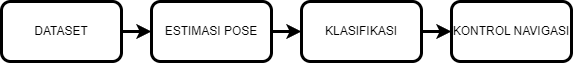
\includegraphics[width=1\linewidth]{../Gambar/metodologi.png}
      \caption{Blok diagram metodologi}
      \label{fig:metodologi}
  \end{figure}

\subsection{Dataset}

Tahapan pengambilan dataset dilakukan dengan mengambilan data-data berupa citra menggunakan kamera pada laptop. Kamera pada laptop dipakai untuk mendapatkan citra yang nantinya digunakan untuk mendeteksi suatu pose atau gestur tangan membutuhkan citra tangan untuk menemukan bagian tangan. Proses pengumpulan citra pose tangan yang digunakan sebagai navigasi robot  dimulai dengan menentukan jumlah kelas dataset. Kelas dataset berjumlah enam pose yang terdiri dari perintah maju, mundur, diam, belok kiri, belok kanan,dan tembak. Setiap pose membutuhkan dua tangan untuk memberikan perintah dengan telapak tangan dihadapkan ke arah kamera. Pose untuk perintah maju dilambangkan dengan kedua tangan mengepal. Pose mundur dilambangkan dengan meluruskan jari manis dan jari tengah seperti halnya pose angka dua pada SIBI pada kedua tangan dan telapak tangan.  Pose diam dilambangkan dengan membuka telapak tangan atau meluruskan semua jari pada kedua tangan.  Pose belok kiri dilambangkan dengan membuka telapak tangan pada tangan kiri dan mengepalkan tangan pada tangan kanan. Pose belok kanan merupakan kebalikan dari pose belok kiri yang dilambangkan dengan tangan kiri mengepal dan tangan kanan membuka telapak tangan. Pose tembak dilambangkan dengan meluruskan ibu jari dan jari manis sedangkan jari lain dikepalkan dengan jari manis diarahkan ke atas dan telapak tangan menghadap ke kamera.

\subsection{Pose Estimation}
Tangan yang terangkap kamera terdeteksi dengan bantuan framework Mediapipe. Framework Mediapipe ini memiliki 21 titik  \emph{keypoint} pada tangan. Proses mendeteksi tangan dimulai dengan cara mencari telapak tangan yang terdapat titik nol \emph{keypoint} yang disebut sebagai palm detection model. Setelah titik nol terdeteksi atau telapak tangan ditemukan kemudian mencari 20 titik lainnya pada tangan. Titik-titik \emph{keypoint} ini dicari menggunakan regresi. Setelah 21 titik \emph{keypoint} terdeteksi selanjutnya menyimpan koordinat x dan y dari yang relatif terhadap layar yang serta menghubungkan 21 titik tersebut sehingga membentuk \emph{hand landmark}. Rangka tiap tangan yang terdeteksi memiliki nilai-nilai koordinat pada tiap \emph{keypoint}, dari koordinat ini dicari nilai terkecil dan nilai terbesar.  Nilai-nilai ini nantinya digunakan untuk membuat bounding box pada setiap frame yang terdeteksi tangan didalamnya. Setiap frame memiliki dua bounding box dikarenakan harus terdapat dua tangan untuk bisa menavigasi robot. Bounding box ini digunakan untuk melakukan hand lokalisasi yang bertujuan untuk menormalisasi variasi posisi dari \emph{hand landmark} yang telah dibuat oleh Mediapipe. Hand lokalisasi ini nantinya membuang bagian citra diluar bounding box dan menyatukan kedua tangan setelahnya. Hasil dari hand lokalisasi nantinya disimpan pada suatu folder pada setiap class. Setelah seluruh data pada setiap class terpenuhi maka dilanjutkan tahapan selanjutnya yaitu \emph{training} dan \emph{classification}.

\subsection{Classification}
Sebelum dilakukannya \emph{classification} dilakukan training data terlebih dahulu. Training data merupakan tahapan dari dataset yang telah dibuat yang kemudian dilatih untuk memperoleh suatu pola dari data tersebut. Pola tersebut digunakan untuk membantu mengenali objek dalam citra. Dalam proses training dibutuhkan konfigurasi yang digunakan. Konfigurasi training yang digunakan yaitu CNN dengan \emph{convolution layer}, \emph{max pooling layer}, dan \emph{fully connected Layer}. Setelah dilakukan proses \emph{validation} dan model yang telah dibuat memiliki akurasi yang tinggi (sesuai dengan \emph{threshold}), maka tahapan selanjutnya yaitu \emph{classification}. Tahap \emph{classification} dilakukan testing menggunakan citra baru lalu dideteksi pose dalam citra tersebut. Citra yang posenya telah diketahui selanjutnya diterjemahkan menjadi kode instruksi yang aka menjadi acuan dalam memberikan perintah kepada robot.

\subsection{Control Navigation}
Tahapan ini berupa cara mengontrol robot menggunakan kode intruksi dari hasil \emph{classification}. Laptop dengan robot terhubung secara \emph{wireless} menggunakan koneksi internet. Hasil \emph{classification} dari laptop dikirimkan kepada robot menggunakan jaringan web socket, dimana laptop dan robot terhubung dalam suatu port dan ip yang telah ditentukan. Robot dapat dikontrol sesuai dari banyaknya \emph{class} pada model yang telah dibuat dalam hal ini terdapat enam \emph{class}. Aksi dari robot ini sesuai dari data yang diterima dari hasil \emph{classification} yakni maju, mundur, kanan, kiri, diam, dan tembak. Tiap-tiap aksi diwakilkan dengan huruf abjad tertentu. Sesuai dengan aksi-aksi tersebut maka robotPergerakan robot dapat terjadi dikarenakan adanya sepasang roda yang dipasangkan pada robot. Perputaran roda diatur dari motor driver dengan menyalurkan listrik kepada motor dc yang sudah dipasangkan roda sebagai outputya. Kemampuan robot untuk tembak menembak menggunakan bantuan \emph{infrared}. Tiap robot nantinya memiliki \emph{infrared} \emph{transmitter} dan \emph{infrared} \emph{receiver} yang diletakkan disekeliling robot. Aksi menembak dimulai dari \emph{infrared} \emph{transmitter} mengirimkan pesan dan nantinya diterima oleh \emph{infrared} \emph{receiver}.

\section{Pengujian dan Pembahasan}
Dalam bab ini dijelaskan mengenai hasil dan pembahasan dari pelaksanaan penelitian, dan juga proses evaluasi pengujiannya. Melalui pembahasan serta pengujian mengenai hasil penelitian, diharapkan dapat menjadi acuan dalam pengambilan kesimpulan dari pelaksanaan tugas akhir ini.

\subsection{Hasil Dataset}
Proses pengumpulan dataset dilakukan dengan pengambilan citra menggunakan kamera. Proses tersebut dilakukan selama beberapa waktu untuk dapat mendapatkan beberapa frame citra untuk suatu class dan diulang kembali dengan class yang berbeda sampai seluruh class terpenuhi. Seluruh citra tangan diambil dari satu orang yang sama dan menggunakan jarak pengambilan yang sama, yaitu jarak antara kamera dan tangan. Dalam proses pengambilan citra dilakukan beberapa variasi dalam pose tangan yaitu dengan sedikit merotasikan tangan dan sedikit melemaskan tangan. Hal ini dilakukan agar tiap class memiliki variasi pose dan dapat mendeteksi dari berbagai kondisi pose. Adapun pose yang digunakan sebagai dataset dapat dilihat pada Tabel \ref{tab:citradaset}.

\begin{table}[H]
    \centering
    \caption{Citra hasil dataset}
    \label{tab:citradaset}
    \begin{tabular}{|c|c|}
    \hline
    Pose   & Citra \\ \hline
    Diam   & 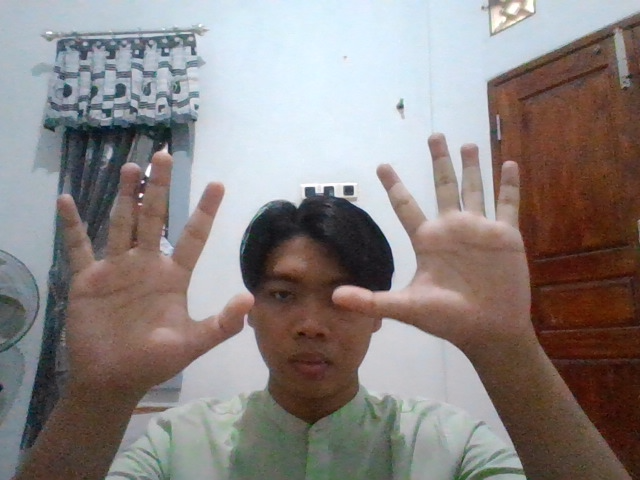
\includegraphics[width=0.3\linewidth]{../Gambar/posediam.png} \\ \hline
    Kanan  & 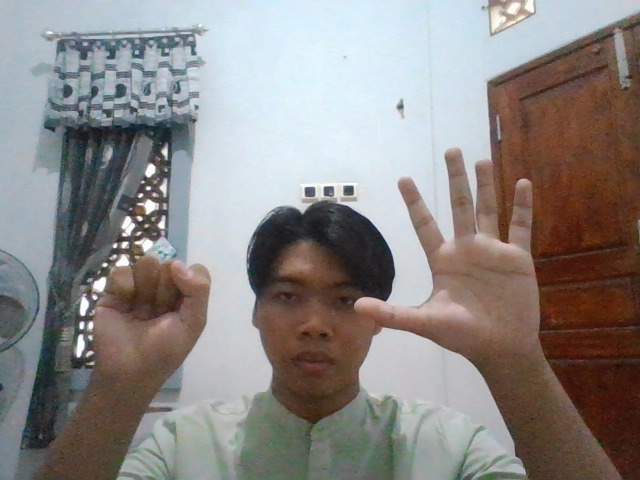
\includegraphics[width=0.3\linewidth]{../Gambar/posekanan.png} \\ \hline
    Kiri   & 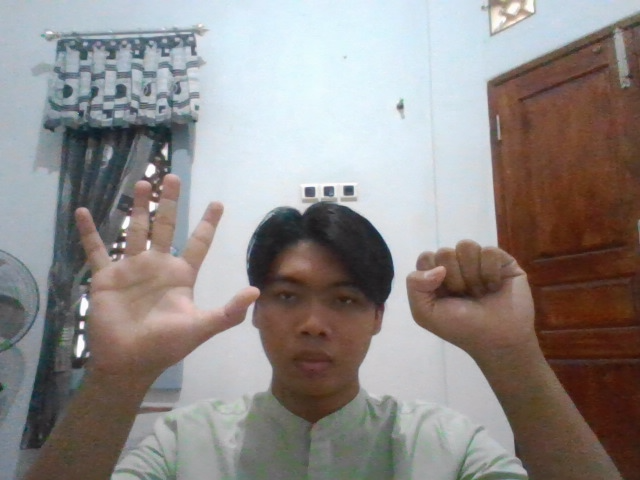
\includegraphics[width=0.3\linewidth]{../Gambar/posekiri.png} \\ \hline
    Maju   & 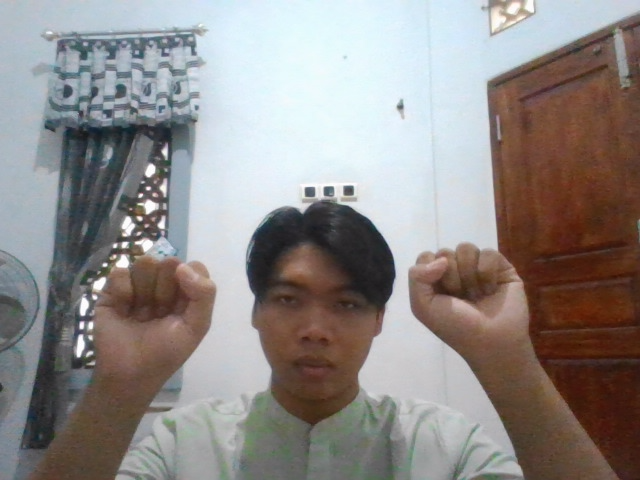
\includegraphics[width=0.3\linewidth]{../Gambar/posemaju.png} \\ \hline
    Mundur & 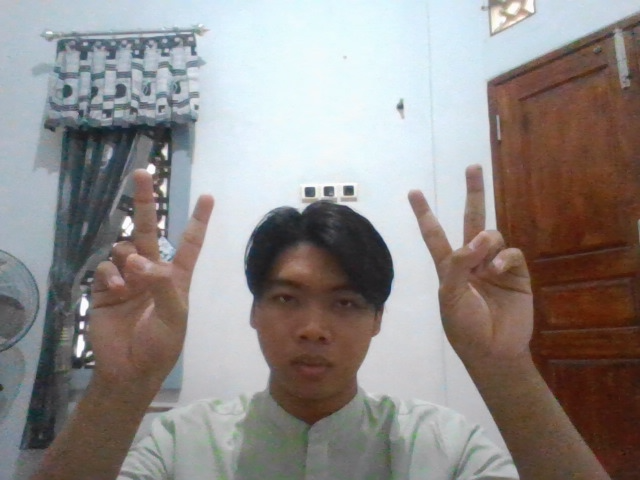
\includegraphics[width=0.3\linewidth]{../Gambar/posemundur.png} \\ \hline
    Tembak & 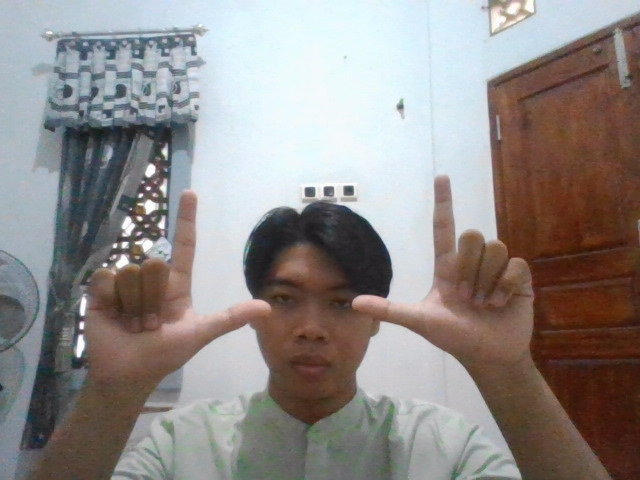
\includegraphics[width=0.3\linewidth]{../Gambar/posetembak.png} \\ \hline
  \end{tabular}
  \end{table}

\subsection{Hasil Pose Estimation}
Proses pose prediction dilakukan dengan menggambar hand landmark yang telah terdeteksi dengan menggunakan Mediapipe pada tiap-tiap citra yang telah dikumpulan pada tahap sebelumnya. Setelah hand landmark tergambar maka tiap-tiap hand landmark digambar pada citra berlatar gelap. Hand landmark yang terdapat pada citra ini diberikan bounding box pada tiap tangan. Setelah bounding box terbuat maka selanjutnya dilakukan hand localization pada hand landmark yang berada pada citra hitam. Hand localization ini untuk mengecilkan ukuran citra menjadi hanya selebar bounding box dengan ditambah 20 pixel pada nilai maksimal dan dikurangi 20 pixel pada nilai minimum pada tiap bounding box. Penambahan pixel ini dimaksudkan untuk mencakup semua hand landmark yang telah dibuat Mediapipe. Dengan mengurangi ukuran citra ini bertujuan mengurangi waktu training dan dapat meningkatkan performa. Citra diluar bounding box dibuang dan tiap bounding box dirubah ukurannya menjadi 128x128 pixel untuk menyamakan kedua bounding box dalam satu frame citra. Setelah setiap ukuran bounding box sama maka setiap bounding box ditumpuk secara horizontal. Citra yang disimpan dan dijadikan dataset adalah citra yang terdapat dua hand landmark yang telah ditumpuk secara horizontal. Citra yang disimpan nantinya memiliki ukuran 256x128 pixel dikarenakan hasil dari dua tangan yang terdeteksi. Pada tahap menumpuk citra terdapat dua macam tumpukan yaitu citra dengan posisi tangan kiri berada pada kotak sebelah kiri dan tangan kanan pada kotak sebelah kanan. Posisi kedua yaitu tangan kiri berada pada posisi kanan dan tangan kanan berada pada kiri yang selanjutnya disebut sebagai posisi invers. Posisi hand landmark dari hasil hand localization dapat dilihat pada Tabel \ref{tab:posisigtangan}.

\begin{table}[H]
    \centering
    \caption{Hasil posisi hand localization}
    \label{tab:posisigtangan}
    \begin{tabular}{|c|c|c|}
    \hline
    Pose   &Pose Benar&Pose Invers\\ \hline
    Diam   & 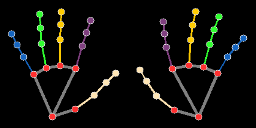
\includegraphics[width=0.3\linewidth]{../Gambar/Diam (1).png} & 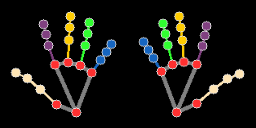
\includegraphics[width=0.3\linewidth]{../Gambar/DiamI (1).png} \\ \hline
    Kanan  & 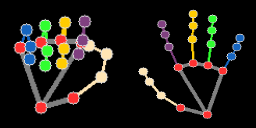
\includegraphics[width=0.3\linewidth]{../Gambar/Kanan (1).png} & 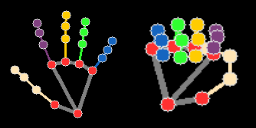
\includegraphics[width=0.3\linewidth]{../Gambar/KananI (1).png} \\ \hline
    Kiri   & 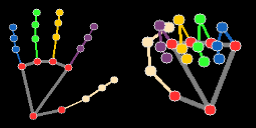
\includegraphics[width=0.3\linewidth]{../Gambar/Kiri (1).png} & 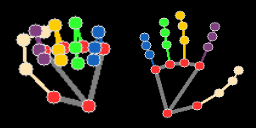
\includegraphics[width=0.3\linewidth]{../Gambar/KiriI (1).png} \\ \hline
    Maju   & 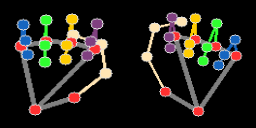
\includegraphics[width=0.3\linewidth]{../Gambar/Maju (1).png} & 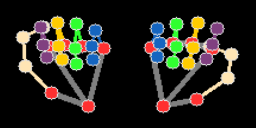
\includegraphics[width=0.3\linewidth]{../Gambar/MajuI (1).png} \\ \hline
    Mundur & 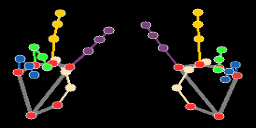
\includegraphics[width=0.3\linewidth]{../Gambar/Mundur (1).png} & 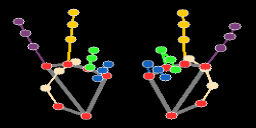
\includegraphics[width=0.3\linewidth]{../Gambar/MundurI (1).png} \\ \hline
    Tembak & 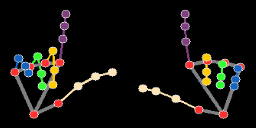
\includegraphics[width=0.3\linewidth]{../Gambar/Tembak (1).png} & 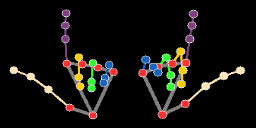
\includegraphics[width=0.3\linewidth]{../Gambar/TembakI (1).png} \\ \hline
    \end{tabular}
  \end{table}

\subsection{Hasil \emph{Classification}}
Proses \emph{classification} dimulai dari \emph{training} dataset. Sebelum melakukan \emph{training} maka dibutuhkannya data citra pada tiap class. Tiap class memiliki \emph{train} data dan \emph{validation} data. Data-data ini diambil dari proses sebelumnya yaitu citra yang telah melewati tahap \emph{hand localization}. Citra untuk train data pada tiap class berjumlah 400 dengan rincian 200 citra posisi benar dan 200 citra posisi invers, sedangkan citra untuk \emph{validation} data berjumlah 80 citra dengan 40 citra posisi benar dan 40 citra posisi invers. Adapaun tabel pesebaran data citra tiap class dapat dilihat pada Tabel \ref{tab:tiapclass}. \emph{Training} ini menggunakan CNN dengan menggunakan satu layer convolution ukuran 3x3 dengan filter 16, sehingga ukuran citra yang awalnya 256x128 turun menjadi 254x126 yang disebabkan dari adanya konvolusi. Selanjutnya dilakukan pooling dengan menggunakan max pooling ukuran 2x2 yang menyebabkan ukuran citra turun menjadi setengah dari hasil konvolusi yaitu 167x63. Layer selanjutnya yaitu flatten dimana citra hasil dari max pooling di ubah menjadi vektor. Output yang didapatkan dari layer flatten yaitu 128016 vektor. Setelah proses konfigurasi layer CNN dan hyperparameter telah dilakukan. Selanjutnya yaitu proses \emph{training} yaitu berupa model dan detail data pada tiap proses pengulangan. Hasil dari \emph{training} ini didapatkan \emph{training accuracy}, \emph{validation accuracy}, \emph{training loss}, dan \emph{validation loss}. Setiap perulangan mendapatkan nilai tersebut, grafik dari nilai tersebut dalam 20 perulangan dapat dilihat pada Gambar \ref{fig:hasiltraining}. Hasil dari \emph{training} didapatkan 
 Evaluasi model menggunakan confusion matrix dengan data testing citra sebanyak 100 pada masing-masing class. Hasil dari confusion matrix didapatkan akurasi 0.95, hasil tersebut secara detail tiap class dapat dilihat pada Gambar \ref{fig:confusionmatrix}.

\begin{figure}[H]
    \centering
    \begin{tabular}{l}
        \multicolumn{1}{c}{\includegraphics[width=0.65\linewidth]{../Gambar/loss.png}} \\
        \multicolumn{1}{c}{a. Grafik \emph{training} dan \emph{validation} \emph{loss}} \\ \\
        \multicolumn{1}{c}{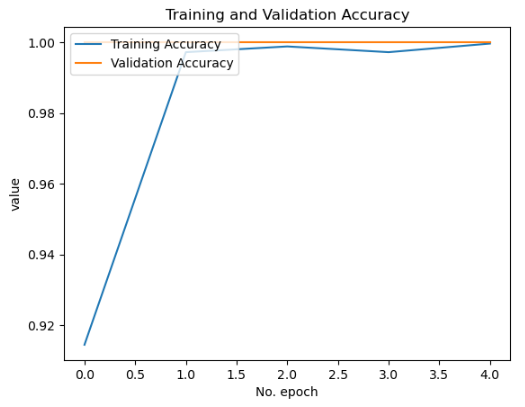
\includegraphics[width=0.65\linewidth]{../Gambar/akurasi.png}} \\
        \multicolumn{1}{c}{b. Grafik \emph{training} dan \emph{validation} \emph{accuracy}} \\   
    \end{tabular}
    \caption{Grafik hasil training}\
    \label{fig:hasiltraining}
\end{figure}

\begin{figure}[H]
  \centering
  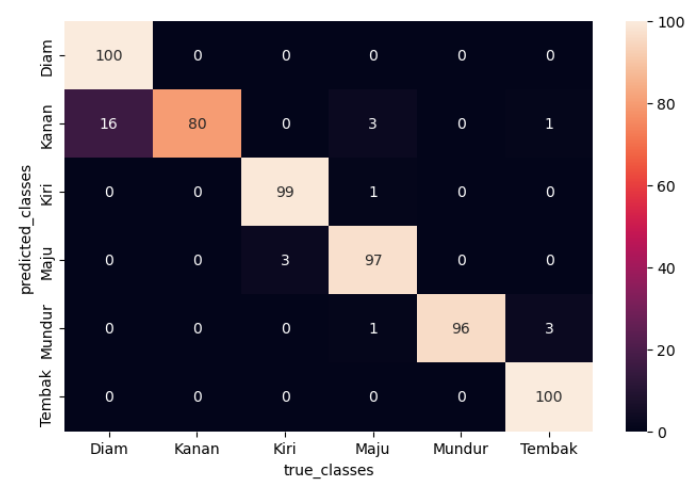
\includegraphics[width=0.7\linewidth]{../Gambar/confusionmatrix.png}
  \caption{Hasil \emph{Confusion Matrix}}
  \label{fig:confusionmatrix}
\end{figure}

\begin{table}[H]
    \centering
    \caption{Jumlah Citra Tiap \emph{Class}}
    \label{tab:tiapclass}
    \begin{tabular}{|c|c|c|}
    \hline
    \emph{Class}  & Train Data & Validation Data \\ \hline
    Diam   & 400        & 80              \\ \hline
    Kanan  & 400        & 80              \\ \hline
    Kiri   & 400        & 80              \\ \hline
    Maju   & 400        & 80              \\ \hline
    Mundur & 400        & 80              \\ \hline
    Tembak & 400        & 80              \\ \hline
    \end{tabular}
  \end{table}

\subsection{Hasil \emph{Control Navigation}}
Proses \emph{control navigation} diawali dengan perancangan pada robot. Robot dirancang dengan memiliki kemampuan untuk bergerak dan menembak. Pergerakan robot dapat terjadi dikarenakan adanya sepasang roda yang dipasangkan pada robot. Perputaran roda diatur dari motor driver dengan menyalurkan listrik kepada motor dc yang sudah dipasangkan roda sebagai outputya. Kemampuan menembak pada robot diatur dengan adanya sensor \emph{infrared}. Sensor \emph{infrared transmitter} diletakkan didepan robot sedangakn sensor \emph{infrared receiver} membutuhkan empat yang diletakkan disekeliling sisi robot. Sensor infrared receiver akan di sambungkan secara pararel untuk ke empat sensornya dan dihubungkan kepada mikrokontroler dalam hal ini yang digunakan adalah "nodeMCU ESP8266". Robot yang telah dirancang selanjutnya diuji dengan cara mengirimkan kode instruksiyang dihasilkan dari proses \emph{classification} kepada mikrokontroler robot. Pengujian ini dilakukan dengan mengklasifikasi 20 citra pada tiap class. Pengujian ini bertujuan untuk mengetahuiapakah ada data yang tidak terkirim atau hilang saat dikirim. Hasil dari klasifikasi akan dirubah menjadi kode instruksi dan dikirim kepada mikrokontroler. Pada mikrokontroler dihitung jumlah kode instruksi yang masuk dan dibandingkan dengan kode yang dikirim. Hasil pengujian ini dapat dilihat pada Tabel \ref{tab:hasulujipose}

\begin{table}[H]
    \centering
    \caption{Hasil uji komunikasi laptop dengan robot}
    \label{tab:hasulujipose}
    \begin{tabular}{|c|c|}
    \hline
    Pose   &  Hasil Uji\\ \hline
    Diam   & 20              \\ \hline
    Kanan  & 20             \\ \hline
    Kiri   & 20              \\ \hline
    Maju   & 20              \\ \hline
    Mundur & 20              \\ \hline
    Tembak & 20              \\ \hline
    \end{tabular}
  \end{table}

\subsection{Hasil Pengujian Jarak}
Pengujian akurasi model bertujuan untuk membandingkan akurasi model dalam beberapa situasi uji guna mengetahui situasi ideal untuk melakukan \emph{classification}. Pengujian ini menggunaka tangan peneliti dengan variasi jarak tangan terhadap kamera dengan ketinggian tangan sejajar dengan kamera. Pengujian jarak dilakukan dengan cara mengambil 20 citra dari tiap class pada jarak tertentu. Jarak ini dimulai dari 30cm, 50cm, 80cm, dan 100cm antara tangan dengan kamera. Pengujian dilakukan karena adanya perubahan bentuk dari \emph{hand landmark}. Hasil pose yang terdeteksi dari pengujian jarak dapat dilihat pada Tabel \ref{tab:hasiljarak}.

\begin{table}[H]
  \centering
  \caption{Pose yang terdeteksi dari pengujian jarak}
  \label{tab:hasiljarak}
  \begin{tabular}{|c|clll|}
    \hline
    \multirow{2}{*}{Pose} & \multicolumn{4}{c|}{Jarak (cm)}                                                   \\ \cline{2-5} 
                          & \multicolumn{1}{l|}{30} & \multicolumn{1}{l|}{50} & \multicolumn{1}{l|}{80} & 100 \\ \hline
    Diam                  & \multicolumn{1}{c|}{20}   & \multicolumn{1}{l|}{19}   & \multicolumn{1}{l|}{20}   &   20  \\ \hline
    Kanan                 & \multicolumn{1}{c|}{20}   & \multicolumn{1}{l|}{20}   & \multicolumn{1}{l|}{16}   &   10  \\ \hline
    Kiri                  & \multicolumn{1}{c|}{18}   & \multicolumn{1}{l|}{20}   & \multicolumn{1}{l|}{20}   &   20  \\ \hline
    Maju                  & \multicolumn{1}{c|}{16}   & \multicolumn{1}{l|}{20}   & \multicolumn{1}{l|}{20}   &   20  \\ \hline
    Mundur                & \multicolumn{1}{c|}{20}   & \multicolumn{1}{l|}{20}   & \multicolumn{1}{l|}{20}   &   20  \\ \hline
    Tembak                & \multicolumn{1}{c|}{20}   & \multicolumn{1}{l|}{20}   & \multicolumn{1}{l|}{15}   &   10  \\ \hline
    Akurasi                  & \multicolumn{1}{c|}{0.95}   & \multicolumn{1}{l|}{0.99}   & \multicolumn{1}{l|}{0.93}   &   0.83  \\ \hline
  \end{tabular}
\end{table}

\begin{thebibliography}{00}
\bibitem{g1} Wibowo, Arif Ardya, Gestur Tangan Manusia dalam Karya Fotografi, Jurnal Fotografi Televisi Animasi, vol 17 No 2, Oktober 2021
\bibitem{g4} Z.Ren, J.Meng, Yuan J. Depth Camera Based Hand Gesture Regconition and its Application in Human-Computer-Interaction. In Processing of the 2011 8th International Conference on Information, Communication and Signal Processing (ICICS). Singapore. 2011.
\bibitem{g3} Hidayatullah Priyanto, Buku Sakti Deep Learning Computer Vision Menggunakan YOLO untuk Pemula, Stunning Vision AI Academy, 2021
\bibitem{g2} Leksono, J. W. and Agung Samudra and Nanndo Yannuansa and Ahmad Fauzi, Kendali mobil robot menggunakan isyarat tangan berbasis arduino, Jurnal Electro Luceat, 2020
\bibitem{g5} Fauzia P. Lestari1, A.B.U. Berlian, M.D.Badrianto, Gesture control car: mengatur gerak mobil hanya dengan memiringkan tangan, 2019
\bibitem{g6} Kukuh Darmawan Setyanto, Ike Fibriani, S.T, M.T., Sumardi, S.T., M.T., PENGENDALIAN MOBILE ROBOT VISION MENGGUNAKAN WEBCAM PADA OBJEK ARAH PANAH BERBASIS RASPBERRY PI, Jurnal Arus Elektro Indonesia (JAEI) 
\bibitem{g7} Hidayatullah, P., Buku sakti deep learning computer vision menggunakan yolo untuk pemula, Stunning Vision AI Academy, 2021
\end{thebibliography}
\end{document}
